
\begin{table}[h]
    \centering
    \small
    \csvautotabular{email.csv}
    \caption{Minimum Dataset for Email Onboarding from Staffbase}
    \label{tab:example_dataset}
\end{table}



In the appendix, we use the example from \cite{nunez2020first} as a demo of querying hybrid provenance.  The dataset is the Minimum Dataset for Email Onboarding(Table \ref{tab:example_dataset}).

We reproduce the data cleaning task with OpenRefine, see Figure \ref{fig:reproduce}. There are five steps in total:

1. We need to extract users' names from 'Login email' without '@' and domain part.

2. We transform data types to numeric in the column Identifier, and as the identifier starts from 0 instead of 1, we delete one each.

3. We add one more column named 'group' based on the value in 'Identifier.' The fourth and fifth is to uppercase the strings in column 'First name' and 'Last name.' 

\begin{figure}
\centering
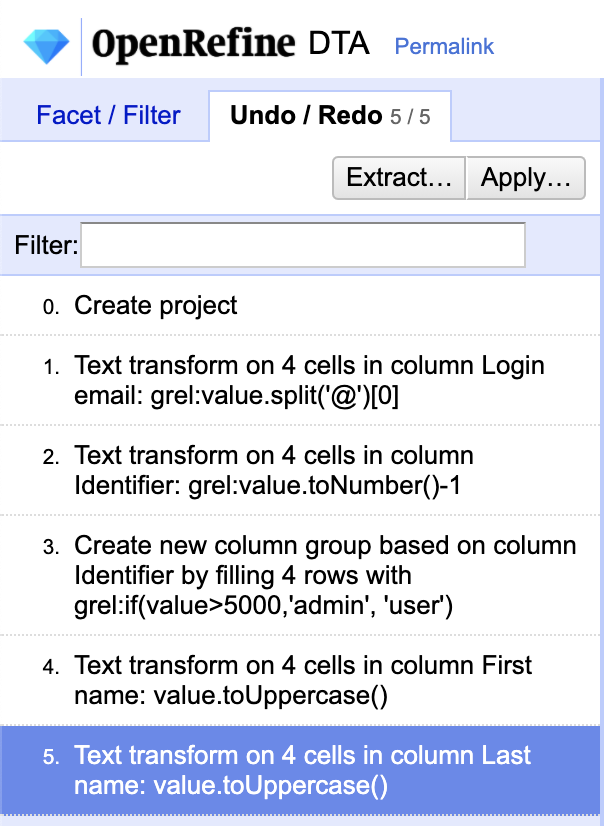
\includegraphics[width=5cm]{Figure/DTA_demo.png}
\caption{Reproduce data cleaning task}
\label{fig:reproduce}
\end{figure}


\subsection{\textbf{The history of three cells}}

We use the query table to reconstruct the operation history of three cells: (1,1), (2,2), and (3,5). According to Table \ref{tab:hybrid_prov}, input the arguments including, hybrid provenance, row index, column index and command $prov-single-cell$, then output the results saving in the result folder, see the Table \ref{tab:DTA_usecase}. (NB: the index starts from 0 in the python program, while for the table, it starts from 1. Therefore, the corresponding provenance is cell at (0,0), (1,1) and (2,4)). 

In the result table \ref{tab:DTA_usecase}, the first column is the cell index, which we want to ask for the provenance. The second column displays the provenance file; the third and fourth columns show the changes of each step. The last column represents the provenance index, which stands for dependency. As we could find, cell at (0,0) and (1,1) are dependent on themselves, while for the cell at (2,4), it has another dependent column. That is because in the data cleaning step 3, this new column 'group,' located in column index 4, is created based on the column $Identifier$, which is located in column index 1.  

In this way, we have verified that hybrid provenance is complete and transparent, providing us with the cell-level changes. On the other side, this query-based provenance helps reveal the dependency information. 

\begin{table}
    \centering
    \begin{tabular}{c|c|c|c|c}
    \hline
    \textbf{Index} & Provenance File & Old Value & New Value & Provenance Index \\
    \hline
    (0,0) & 'hybrid1' & 'laura@example.com' & 'laura' & (0,0) \\
    \hline
    (1,1) & 'hybrid2' & ' 4081'& 4080 & (1,1) \\
    \hline
    (2,4) & 'hybrid2' & ' 9346' & 9345 & (2,1) \\
     & 'hybrid3' & None & 'admin' & (2,4) \\
    \hline
    \end{tabular}
    \caption{Result of Provenance for three cells}
    \label{tab:DTA_usecase}
\end{table}





\footnote{See: \url{https://github.com/LanLi2017/X_or2yw}}